\documentclass[aspectratio=169]{beamer}
\usepackage{amsmath}
\usepackage{amssymb}
\usepackage{minted}
\usepackage{graphicx}
\title{EM algorithm}
\subtitle{Maximum Likelihood Estimation of the t-distribution}
\author{Lucas Støjko Andersen}
\setminted{fontsize=\fontsize{8pt}{8pt}}
\institute{University of Copenhagen}
\date{\today}

\begin{document}
\begin{frame}
    \titlepage
\end{frame}
\begin{frame}
    \frametitle{The t-distribution}
    \framesubtitle{The density of the non-standard t-distribution}
    The density of the t-distribution is given by
    \begin{equation}
        \label{eq:marginal}
        g(x)=\frac{\Gamma\left(\frac{\nu + 1}{2}\right)}{\sqrt{\pi\nu\sigma^2}\Gamma\left(\frac{\nu}{2}\right)}\left(1+\frac{(x - \mu)^2}{\nu\sigma^2}\right)^{-\frac{\nu + 1}{2}}
    \end{equation}
    with parameters $\mu\in\mathbf{R}$, $\nu > 0$, $\sigma^2 > 0$. Here, $\Gamma$ is the gamma function.\\[12pt]
    For independent observations $X_{1},X_{2},\ldots,X_{n}$ with density as in (\ref{eq:marginal}) there exist no nice analytic solutions to the MLE --- even with $\nu$ known.
\end{frame}
\begin{frame}
    \frametitle{There is another way}
    \framesubtitle{A joint approach with latent variables}
    Consider $(X, W)$ with density
    \begin{equation}
        \label{eq:join}
        f(x,w)=\frac{1}{\sqrt{\pi\nu\sigma^2}2^{(\nu+1)/2}\Gamma(\nu/2)}w^{\frac{\nu - 1}{2}}e^{-\frac{w}{2}\left(1+\frac{(x -\mu)^2}{\nu\sigma^2}\right)}
    \end{equation}
    Notice that $W\mid X = x \sim \Gamma(\alpha, \beta)$ --- the gamma distribution --- with parameters
    \begin{equation}
        \alpha = \frac{\nu + 1}{2} \quad\quad 
        \beta = \frac{1}{2}\left(1+\frac{(x -\mu)^2}{\nu\sigma^2}\right).
    \end{equation}
    This can be used to show that $X$ indeed has the marginal density of the t-distribution with parameters $\mu,\sigma^2,\nu$.
\end{frame}
\begin{frame}
    \frametitle{The Full Maximum Likelihood Estimate}
    \framesubtitle{MLE with fixed $\nu$}
    Assume $\nu>0$ known. I.i.d. $(X_{1},W_{1}), (X_{2},W_{2}),\ldots,(X_{n},W_{n})$ have log-likelihood
    \begin{equation}
        \ell(\theta)\simeq -\frac{n}{2}\log\sigma^2 -\frac{1}{2\nu\sigma^2}\sum_{i=1}^{n}W_{i}(X_{i}-\mu)^{2}.
    \end{equation}
    The solution is that of the weighted least squares:
    \begin{equation}
        \hat\mu =\frac{\sum_{i=1}^{n}W_{i}X_{i}}{\sum_{i=1}^{n}W_{i}},\quad\quad \hat\sigma^2 = \frac{1}{n\nu}\sum_{i=1}^{n}W_{i}(X_{i}-\hat\mu)^{2}.
    \end{equation}
\end{frame}
\begin{frame}
    \frametitle{EM algorithm}
    \framesubtitle{MLE of the marginal likelihood for fixed $\nu$}
    Only $X$ is observed and so the full MLE cannot be computed. Using the EM algorithm we iteratively maximize the quantity
    \begin{equation}
        Q(\theta\mid\theta')=E_{\theta'}(\log f_{\theta}(X, W)\mid X)
    \end{equation}
    where $\theta = (\mu,\sigma^2)$. Using the log-likelihood from earlier
    \begin{equation}
        Q(\theta\mid\theta')\simeq -\frac{n}{2}\log\sigma^{2}-\frac{1}{2\nu\sigma^{2}}\sum_{i=1}^{n}E_{\theta'}(W_{i}\mid X_{i})(X_{i}-\mu)^{2}.
    \end{equation}
    The maximizer is then
    \begin{equation*}
        \hat\mu_{\theta'} =\frac{\sum_{i=1}^{n}E_{\theta'}(W_{i}\mid X_{i})X_{i}}{\sum_{i=1}^{n}E_{\theta'}(W_{i}\mid X_{i})},\quad \hat\sigma^{2}_{\theta'}= \frac{1}{n\nu}\sum_{i=1}^{n}E_{\theta'}(W_{i}\mid X_{i})(X_{i}-\hat\mu_{\theta'})^{2}.
    \end{equation*}
\end{frame}
\begin{frame}
    \frametitle{EM algorithm}
    \framesubtitle{E-step and M-step}
    The E-step boils down to computing $E_{\theta'}(W_{i} \mid X_{i})$
    \begin{equation}
        E_{\theta'}(W_{i} \mid X_{i}) = \frac{\alpha}{\beta}=\frac{\nu' + 1}{2}\frac{1}{\frac{1}{2}\left(1 + \frac{(X_{i} - \mu')^{2}}{\nu'\sigma'^{2}}\right)}=\frac{\nu' + 1}{1 + \frac{(X_{i}- \mu')^{2}}{\nu'\sigma'^{2}}}
    \end{equation}
    and doing the M-step by computing
    \begin{equation*}
        \hat\mu_{\theta'} =\frac{\sum_{i=1}^{n}E_{\theta'}(W_{i}\mid X_{i})X_{i}}{\sum_{i=1}^{n}E_{\theta'}(W_{i}\mid X_{i})},\quad \hat\sigma^{2}_{\theta'}= \frac{1}{n\nu}\sum_{i=1}^{n}E_{\theta'}(W_{i}\mid X_{i})(X_{i}-\hat\mu_{\theta'})^{2}.
    \end{equation*}
\end{frame}
\begin{frame}[fragile]
    \frametitle{Implementation of EM-algorithm}
\begin{minted}{r}
EM <- function(x, nu, cb = NULL, maxit = 500L, min.eps = 1e-7, par = NULL) {
  if(is.null(par)) par <- c(median(x), IQR(x))
  par1 <- numeric(2)
  n <- length(x)
  EW <- numeric(n)
  for(i in 1:maxit) {
    EW <- (nu + 1) / (1 + ((x - par[1])^2) / (nu * par[2]))
    par1[1] <- sum(EW * x) / sum(EW)
    par1[2] <- sum(EW * (x - par[1])^2) / (n * nu)
    if(!is.null(cb)) cb()
    if(norm(par - par1, "2") < min.eps * (norm(par1, "2") + min.eps)) break
    par <- par1
  }
  if(i == maxit) warning("Maximum number of itertaions ", maxit, " reached.")
  names(par1) <- c("mu", "sigma")
  list(par = par1, iterations = i, nu = nu)
}
\end{minted}
\end{frame}
\begin{frame}[fragile]
    \frametitle{Implementation of the Newton Algorithm}
\begin{minted}{r}
Newton <- function(par, H, gr, hess,
                   d = 0.8, c = 0.2, gamma0 = 1, 
                   min.eps = 1e-7, maxit = 500L, cb = NULL) {
  for(i in 1:maxit) {
    value <- H(par)
    grad <- gr(par)
    Hessian <- hess(par) 
    rho <- - drop(solve(Hessian, grad)) 
    gamma <- gamma0
    par1 <- par + gamma * rho
    h_prime <- crossprod(grad, rho)
    while(min(H(par1), Inf, na.rm = TRUE) > value +  c * gamma * h_prime) { 
      gamma <- d * gamma 
      par1 <- par + gamma * rho
    }
    if(!is.null(cb)) cb()
    if(norm(par - par1, "2") < min.eps * (norm(par1, "2") + min.eps)) break 
    par <- par1 
  }
  if(i == maxit) warning("Maximal number, ", maxit, ", of iterations reached")
  list(par = par1, iterations = i)
}
\end{minted}
\end{frame}
\begin{frame}
    \frametitle{Comparison}
    Simulate 10.000 samples from a t-distribution with parameters $\mu = 5$, $\sigma^{2}=3$ and $\nu = 2.5$ and 10.000 samples with $\nu = 0.5$.   
    \begin{figure}
        \centering
        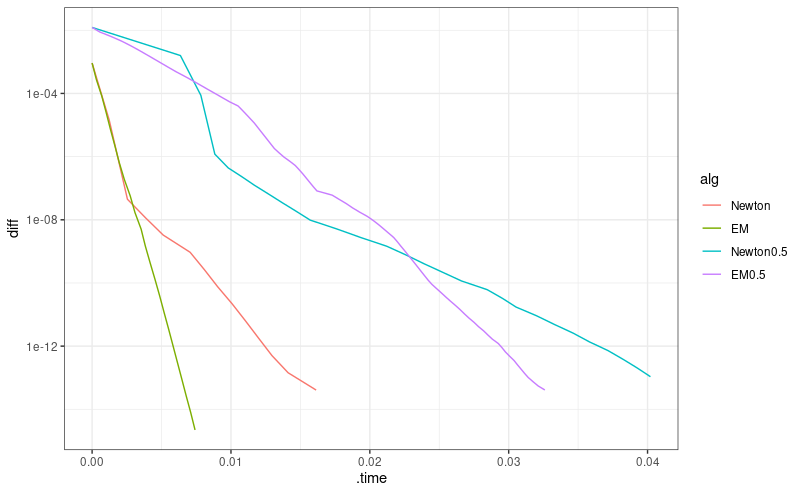
\includegraphics[scale = 0.4]{figure/R_NewtonVsEm.png}
    \end{figure}
\end{frame}
\begin{frame}
    \frametitle{Comparison}    
    \framesubtitle{Benchmarks Using \texttt{bench} Package}
    \begin{figure}
        \centering
        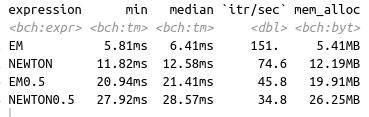
\includegraphics[scale = 0.6]{figure/R_NewtonVsEm_table.png}
    \end{figure}
\end{frame}
\begin{frame}
    \frametitle{Profiling of the Newton Algorithm Implementation}
    Using 100.000 samples.
    \begin{figure}
        \centering
        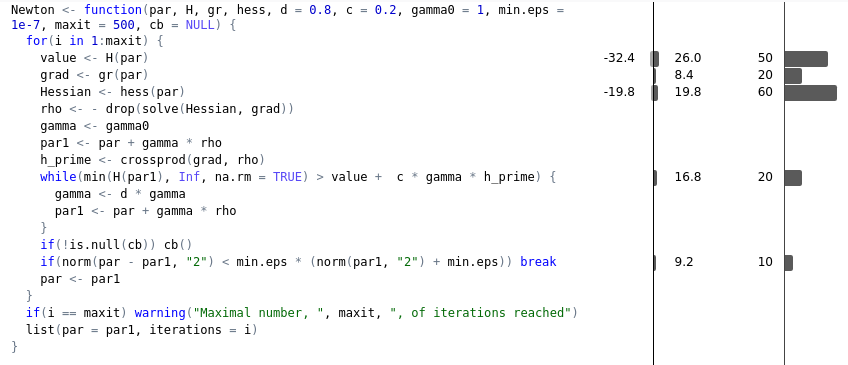
\includegraphics[scale = 0.4]{figure/NewtonProfile.png}
    \end{figure}
\end{frame}
\begin{frame}[fragile]
    \frametitle{Profiling of the Newton Algorithm}
    \framesubtitle{Implementation of Log-likelihood and Gradient}
\begin{minted}[fontsize = \fontsize{7pt}{7pt}]{r}
get_like <- function(x, nu) {
  n <- length(x); force(nu)
  function(par) {
    mu <- par[1]; sigma <- par[2]
    K <- sum(log(1 + (x - mu)^2 / (nu * sigma)))
    log(sigma) / 2 + (nu + 1) * K / (2 * n)
  }
}

get_grad <- function(x, nu) {
  n <- length(x); force(nu)
  function(par) {
    mu <- par[1]; sigma <- par[2]
    C1 <- (x - mu) / (1 + (x - mu)^2 / (nu * sigma))
    K_mu <- sum(C1)
    K_sigma <- sum(C1 * (x - mu))
    grad_mu <- -(nu + 1) * K_mu / (n * nu * sigma)
    grad_sigma <- 1 / (2 * sigma) - (nu + 1) * K_sigma / (2 * n * nu * sigma^2)
    c(grad_mu, grad_sigma)
  }
}
\end{minted}
\end{frame}
\begin{frame}[fragile]
    \frametitle{Implementation of Log-likelihood, Gradient and Hessian Using \texttt{Rcpp}}
\begin{minted}{cpp}
// [[Rcpp::export]]
double CPP_likelihood(NumericVector par, NumericVector x, double nu) {
  double K = sum(log(1 + (x - par[0]) * (x - par[0]) / (nu * par[1])));
  return log(par[1]) / 2 + (nu + 1) * K / (2 * x.size());
}

// [[Rcpp::export]]
NumericVector CPP_gradient(NumericVector par, NumericVector x, double nu) {
  int n = x.size();
  double K_mu = 0, K_sigma = 0;
  for(int i = 0; i < n; ++i) {
    double C1 = (x[i] - par[0]) / 
      (1 + (x[i] - par[0]) * (x[i] - par[0]) / (nu * par[1]));
    K_mu += C1;
    K_sigma += C1 * (x[i] - par[0]);
  }
  NumericVector grad(2);
  grad[0] = -(nu + 1) * K_mu / (n * nu * par[1]);
  grad[1] = 1 / (2 * par[1]) - 
    (nu + 1) * K_sigma / (2 * n * nu * par[1] * par[1]);
  return grad;
}
\end{minted}
\end{frame}
\begin{frame}[fragile]
    \frametitle{Implementation of Log-likelihood, Gradient and Hessian Using \texttt{Rcpp}}
\begin{minted}{cpp}
// [[Rcpp::export]]
NumericMatrix CPP_hessian(NumericVector par, NumericVector x, double nu) {
  int n = x.size();
  double K1 = 0, K2 = 0, K3 = 0, K4 = 0, K5 = 0, K6 = 0;
  for(int i = 0; i < n; ++i) {
    double C0 = 1 / (1 + (x[i] - par[0]) * (x[i] - par[0]) / (nu * par[1]));
    double C1 = C0 * (x[i] - par[0]);
    double C2 = C1 * (x[i] - par[0]);
    K1 += C0;
    K2 += C1;
    K3 += C1 * C1;
    K4 += C2;
    K5 += C2 * C2;
    K6 += C1 * C1 * (x[i] - par[0]);
  }
  NumericMatrix hess(2, 2);
  hess(0, 0) = (nu + 1) * K1 / (n * nu * par[1]) +
    2 * (nu + 1) * K3 / (n * nu * nu * par[1] * par[1]);
  hess(0, 1) = (nu + 1) * K2 / (n * nu * par[1] * par[1]) -
    (nu + 1) * K6 / (n * nu * par[1] * par[1] * par[1]);
  hess(1, 0) = hess(0, 1);
  hess(1, 1) = -1 / (2 * par[1] * par[1]) +
    (nu + 1) * K4 / (n * nu * par[1] * par[1] * par[1]) -
    (nu + 1) * K5 / (2 * n * nu * nu * par[1] * par[1] * par[1] * par[1]);
  return hess;
}
\end{minted}
\end{frame}
\begin{frame}
    \frametitle{Benchmarks of New Log-likelihood, Gradient and Hessian}    
    \begin{figure}
        \centering
        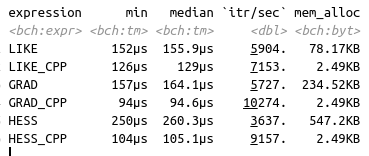
\includegraphics[scale = 0.6]{figure/CPP_LogGrHess.png}
    \end{figure}
\end{frame}
\begin{frame}
    \frametitle{Benchmarks of New Log-likelihood, Gradient and Hessian}
    \begin{figure}
        \centering
        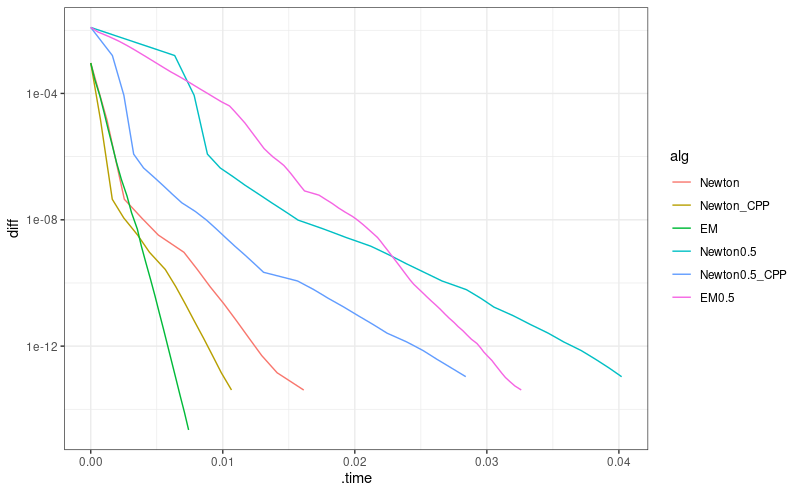
\includegraphics[scale = 0.5]{figure/CPPN_NewtonVsEm.png}
    \end{figure}
\end{frame}
\begin{frame}
    \frametitle{Benchmarks of New Log-likelihood, Gradient and Hessian}
    \begin{figure}
        \centering
        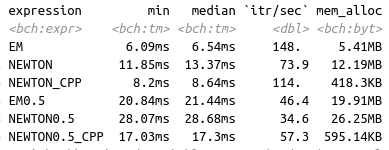
\includegraphics[scale = 0.6]{figure/CPPN_NewtonVsEm_table.png}
    \end{figure}
\end{frame}
\begin{frame}[fragile]
    \frametitle{\texttt{Rcpp} Implementation of EM-algorithm}
\begin{minted}[fontsize = \fontsize{7pt}{7pt}]{cpp}
double dist(double x1, double x2, double y1, double y2) {
  double x_sq = x1 * x1 + x2 * x2;
  double y_sq = y1 * y1 + y2 * y2;
  double xy = x1 * y1 + x2 * y2;
  return std::sqrt(x_sq + y_sq - 2 * xy);
}

// [[Rcpp::export]]
List CPP_EM(NumericVector par0, 
                    NumericVector x, 
                    double nu,
                    int maxit,
                    double eps) {
  int n = x.size();
  NumericVector par = clone(par0);
  NumericVector par1(2);
  int i;
  for(i = 0; i < maxit; ++i) {
    NumericVector EW = (nu + 1) / 
      (1 + (x - par[0]) * (x - par[0]) / (nu * par[1]));
    par1[0] = sum(EW * x) / sum(EW);
    par1[1] = sum(EW * (x - par[0]) * (x - par[0])) / (n * nu);
    double norm_new = dist(par[0], par[1], par1[0], par1[1]);
    double norm_old = std::sqrt(par1[0] * par1[0] + par1[1] * par1[1]);
    if(norm_new < eps * (norm_old + eps)) break;
    par[0] = par1[0];
    par[1] = par1[1];
  }
  if(i != maxit) i += 1;
  return List::create(par1, i);
}
\end{minted}
\end{frame}
\begin{frame}[fragile]
    \frametitle{Implementation of Newton Algorithm Using \texttt{R}'s C Interface}
\begin{columns}
\begin{column}{0.5\textwidth}
\begin{minted}[fontsize = \fontsize{6pt}{6pt}]{c}
SEXP C_Newton(SEXP par0, SEXP H, SEXP gr, SEXP hess,
              SEXP d, SEXP c, SEXP gamma0, 
              SEXP eps, SEXP maxit,
              SEXP env) {
  int n = length(par0), info;
  SEXP H_call = PROTECT(lang2(H, R_NilValue));
  SEXP gr_call = PROTECT(lang2(gr, R_NilValue));
  SEXP hess_call = PROTECT(lang2(hess, R_NilValue));
  SEXP value, grad, hessian, Hpar;
  SEXP par = PROTECT(allocVector(REALSXP, n));
  SEXP par1 = PROTECT(allocVector(REALSXP, n));
  double value_, *grad_, *hessian_; 
  double *par1_ = REAL(par1), *par_ = REAL(par);
  double gamma0_ = REAL(gamma0)[0], d_ = REAL(d)[0], c_ = REAL(c)[0];
  double eps_ = REAL(eps)[0], maxit_ = INTEGER(maxit)[0];
  double *rho = (double*)malloc(sizeof(double) * n);
  
  for(int i = 0; i < n; ++i)
    REAL(par)[i] = REAL(par0)[i];
  int k;
  
  for(k = 0; k < maxit_; ++k) {
    double gamma = gamma0_;
    double h_prime;
    SETCADR(H_call, par);
    value = PROTECT(eval(H_call, env));
    SETCADR(gr_call, par);
    grad = PROTECT(eval(gr_call, env));
    SETCADR(hess_call, par);
    hessian = PROTECT(eval(hess_call, env));
    hessian_ = REAL(hessian);
    grad_ = REAL(grad);
\end{minted}
\end{column}
\begin{column}{0.5\textwidth}
\begin{minted}[fontsize = \fontsize{6pt}{6pt}]{c}
  for(int j = 0; j < n; ++j)
    grad_[j] = -grad_[j];
  value_ = REAL(value)[0];
  solve(n, hessian_, grad_, rho, &info);
  if(info != 0) break;
  for(int j = 0; j < n; ++j) {
    par1_[j] = par_[j] + gamma * rho[j];
    h_prime += grad_[j] * rho [j];
  }
  while(1 == 1) {
    SETCADR(H_call, par1);
    Hpar = eval(H_call, env);
    if(ISNAN(REAL(Hpar)[0]) || 
        REAL(Hpar)[0] > value_ + c_ * gamma * h_prime) {
      gamma = d_ * gamma;
      for(int j = 0; j < n; ++j)
        par1_[j] = par_[j] + gamma * rho[j];
    } else break;
  }
  UNPROTECT(3);
  double norm = norm2(par1_, n);
  for(int j = 0; j < n; ++j)
    par_[j] -= par1_[j];
  double norm_new = norm2(par_, n);
  if(norm_new < eps_ * (norm + eps_)) break;
  for(int j = 0; j < n; ++j) {
    par_[j] = par1_[j];
  }
}
\end{minted}
\end{column}
\end{columns}
\end{frame}
\begin{frame}[fragile]
    \frametitle{Implementation of Newton Algorithm Using \texttt{R}'s C Interface}
    \framesubtitle{Continued}
\begin{minted}{c}
  SEXP result = PROTECT(allocVector(VECSXP, 2));
  SET_VECTOR_ELT(result, 0, par1);
  if(k != maxit_) k += 1;
  if(info != 0) {
    SET_VECTOR_ELT(result, 1, ScalarInteger(-1));
  } else {
    SET_VECTOR_ELT(result, 1, ScalarInteger(k));
  }
  UNPROTECT(6);
  free(rho);
  return result;
}
\end{minted}
\end{frame}
\begin{frame}[fragile]
    \frametitle{Implementation of Newton Algorithm Using \texttt{R}'s C Interface}
\begin{minted}{c}
double norm2(double *x, int m) {
  char jobu = 'N', jobvt = 'N';
  int n = 1, info, lwork;
  if(m > 3) {
    lwork = m + 2;
  } else {
    lwork = 5;
  }
  double U, VT, s;
  double *A = (double*)malloc(sizeof(double) * m);
  double *work = (double*)malloc(sizeof(double) * lwork);
  for(int i = 0; i < m; ++i)
    A[i] = x[i];
  dgesvd_(&jobu, &jobvt, &m, &n, A, &m, &s, 
          &U, &m, &VT, &m, work, &lwork, &info);
  free(A);
  free(work);
  return s;
}

void solve(int n, double *a, double *b, double *result, int *info) {
  for(int i = 0; i < n; ++i)
    result[i] = b[i];
  int nrhs = 1;
  int *ipiv = (int*)malloc(sizeof(int) * n);
  dgesv_(&n, &nrhs, a, &n, ipiv, result, &n, info);
  free(ipiv);
}
\end{minted}
\end{frame}
\begin{frame}[fragile]
    \frametitle{Wrappers}    
\begin{minted}{r}
Newton_C <- function(par, H, gr, hess, 
                     d = 0.8, c = 0.2, gamma0 = 1, 
                     min.eps = 1e-7, maxit = 500) {
  result <- .Call("C_Newton",
                  par,
                  H,
                  gr,
                  hess,
                  d,
                  c,
                  gamma0,
                  min.eps,
                  as.integer(maxit),
                  environment())
  if(result[[2]] == -1L)
    warning("Matrix solve went wrong.")
  if(result[[2]] == maxit)
    warning("Maximal number, ", maxit, ", of iterations reached")
  list(par = result[[1]], iterations = result[[2]])
}
\end{minted}
\end{frame}
\begin{frame}[fragile]
    \frametitle{Wrappers}
\begin{minted}{r}
EM_cpp <- function(par = NULL, x, nu, cb = NULL, maxit = 500, min.eps = 1e-7) {
  if(is.null(par)) par <- c(median(x), IQR(x))
  par1 <- numeric(2)
  n <- length(x)
  EW <- numeric(n)
  result <- CPP_EM(par, x, nu, maxit, min.eps)
  if(result[[2]] == maxit) warning("Maximum number of itertaions ", maxit, " reached.")
  names(result[[1]]) <- c("mu", "sigma")
  list(par = c(result[[1]]), 
       iterations = result[[2]], 
       nu = nu)
}
\end{minted}
\end{frame}
\begin{frame}
    \frametitle{Final Benchmarks}
    \begin{figure}
        \centering
        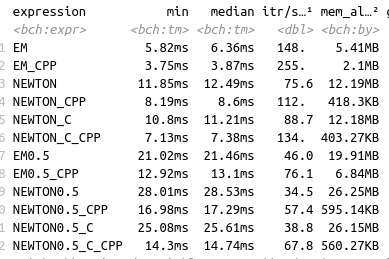
\includegraphics[scale = 0.6]{figure/C_NewtonVsEm.png}
    \end{figure}
\end{frame}
\begin{frame}[fragile]
    \frametitle{Appendix}
    \framesubtitle{Final Implementation}   
\begin{minted}{r}
EM_cpp <- function(par = NULL, x, nu, cb = NULL, maxit = 500, min.eps = 1e-7) {
  if(is.null(par)) par <- c(median(x), IQR(x))
  par1 <- numeric(2)
  n <- length(x)
  EW <- numeric(n)
  result <- CPP_EM(par, x, nu, maxit, min.eps)
  if(result[[2]] == maxit) warning("Maximum number of itertaions ", maxit, " reached.")
  names(result[[1]]) <- c("mu", "sigma_sq")
  structure(
    list(par = c(result[[1]]), 
         iterations = result[[2]], 
         nu = nu, 
         x = x),
    class = "em_estimate"
    )
}
\end{minted}
\end{frame}
\begin{frame}[fragile]
    \frametitle{Appendix}
    \framesubtitle{Final Implementation}
\begin{minted}[fontsize = \fontsize{7pt}{7pt}]{r}
EM_fisher <- function(mle, x, nu) {
  Q <- Q_func(x, nu, mle)
  phi <- phi_func(x, nu)
  IY <- numDeriv::hessian(Q, mle)
  IX <- (diag(1, 2) - t(numDeriv::jacobian(phi, mle))) %*% IY
  solve(IX)
}

Q_func <- function(x, nu, mle) {
  force(x); force(nu); force(par);
  function(par) Q_cpp(par, mle, x, nu)
}

phi_func <- function(x, nu) {
  force(x); force(nu)
  function(par) phi_cpp(par, x, nu)
}

confint.em_estimate <- function(x, level = 0.95) {
  qq <- level + (1 - level) / 2
  qq <- qnorm(qq)
  invf <- EM_fisher(x$par, x$x, x$nu)
  mu <- x$par[1] + c(-1, 1) * qq * sqrt(invf[1, 1])
  sigma <- x$par[2] + c(-1, 1) * qq * sqrt(invf[2, 2])
  names(mu) <- c("lwr", "upr")
  names(sigma) <- c("lwr", "upr")
  list(mu = mu, sigma_sq = sigma)
}
\end{minted}
\end{frame}
\begin{frame}[fragile]
    \frametitle{Appendix}
    \framesubtitle{Final Implementation}
\begin{minted}[fontsize = \fontsize{7pt}{7pt}]{cpp}
// [[Rcpp::export]]
NumericVector phi_cpp(NumericVector par0,
                      NumericVector x,
                      double nu)  {
  int n = x.size();
  NumericVector par(2);
  NumericVector EW = (nu + 1) / 
    (1 + (x - par0[0]) * (x - par0[0]) / (nu * par0[1]));
  
  par[0] = sum(EW * x) / sum(EW);
  par[1] = sum(EW * (x - par[0]) * (x - par[0])) / (n * nu);
  
  return par;
}

// [[Rcpp::export]]
double Q_cpp(NumericVector par,
              NumericVector par1,
              NumericVector x,
              double nu) {
  
  int n = x.size();
  double value = 0.5 * log(par[1]) * n;
  NumericVector C2 = (nu + 1) / 
    (1 + (x - par1[0]) * (x - par1[0]) / (nu * par1[1]));
  return value + sum(C2 * (x - par[0]) * (x - par[0]) / (2 * nu * par[1]));
}
\end{minted}
\end{frame}
\begin{frame}[fragile]
    \frametitle{Appendix}
    \framesubtitle{Full \texttt{RcppArmadillo} Implementation of Newton Algorithm}
\begin{minted}[fontsize = \fontsize{5pt}{5pt}]{cpp}
// [[Rcpp::export]]
List FitT(NumericVector par0, NumericVector x, double nu, double c,
          double d, double gamma0, int maxit, double eps) {
  
  arma::mat::fixed<2, 2> hess;
  arma::vec::fixed<2> grad;
  arma::vec::fixed<2> p1;
  arma::vec::fixed<2> p2;
  NumericVector par1(2), par = clone(par0);
  int n = x.size();
  int i;
  for(i = 0; i < maxit; ++i) {
    double value = CPP_likelihood(par, x, nu);
    NumericVector gr = CPP_gradient(par, x, nu);
    NumericMatrix hessian = CPP_hessian(par, x, nu);
    grad[0] = gr[0], grad[1] = gr[1];
    hess(0, 0) = hessian(0, 0), hess(0, 1) = hessian(0, 1);
    hess(1, 0) = hessian(1, 0), hess(1, 1) = hessian(1, 1);
    arma::vec::fixed<2> rho = -arma::solve(hess, grad);
    double gamma = gamma0;
    par1[0] = par[0] + gamma * rho[0];
    par1[1] = par[0] + gamma * rho[1];
    double h_prime = rho[0] * gr[0] + rho[1] * gr[1];
    while(CPP_likelihood(par1, x, nu) > value + c * gamma * h_prime) {
      gamma *= d;
      par1[0] = par[0] + gamma * rho[0];
      par1[1] = par[1] + gamma * rho[1];
    }
    p1[0] = par1[0], p1[1] = par1[1];
    p2[0] = par1[0] - par[0], p2[0] = par1[1] - par[1];
    double norm = arma::norm(p1, 2);
    double norm_new = arma::norm(p2, 2);
    if(norm_new < eps * (norm + eps)) break;
    par[0] = par1[0], par[1] = par1[1];
  }
  if(i != maxit) i -= 1;
  NumericVector iter(1);
  iter[0] = i;
  return List::create(par1, iter);
}
\end{minted}
\end{frame}
\end{document}
